\documentclass{article}
\usepackage[utf8]{inputenc}
\usepackage{graphicx}


\title{CMSC 6950 Final Project - eddy}
\author{Khalid Ibne Hasan }
\date{June 2021}

\begin{document}

\maketitle

\section{Introduction}
The aim of this project was to select a project topic from the list of JOSS papers and perform two computational tasks along with two visualizations. The name of the chosen software package is eddy, which implements several methods for extracting kinematical information from astronomical observations of Doppler shifted molecular line emission in protoplanetary disks \cite{Teague2019}. The package further implements methods to fit a first moment map that is a frequently used analysis in the study of protoplanetary disks, typically used to constrain the mass of the central star and extract geometrical properties. Two visualizations followed by two computational tasks have been carried out for this project using the eddy software package, astropy, numpy and matplotlib.

\section{Results}
In this section, the results obtained from the computational tasks and their visualizations will be discussed. The tasks are dependant on line-of-sight velocity maps made through bettermoments available at eddy dataverse. Initially, the first task produces an image reading the map data of the FITS file and takes the help of the software package to generate a downsampled and clipped rotation map. In the second task, the rotation map is fit to infer their geometrical properties, such as the source center, position angle, stellar mass, and the system velocity at a fixed inclination of 6.8 degrees. 
\subsection{Task 1: Load Data and Plot Rotation Map}
For this task, two primary datasets of CO J = 2-1 emission around TW Hydra star and CO J = 2-1 emission around HD 163296 circumstellar disk have been used to load the data. The first computation produces an image representing the data from the datasets and then generates a more optimized rotation map. The loaded data is saved into an intermediate file using pickle, which will be used in later computational tasks. The intermediate file is imported into another python script to generate the plot of the rotation map further. 
\begin{figure}
\caption{FITS Image of TW Hya}
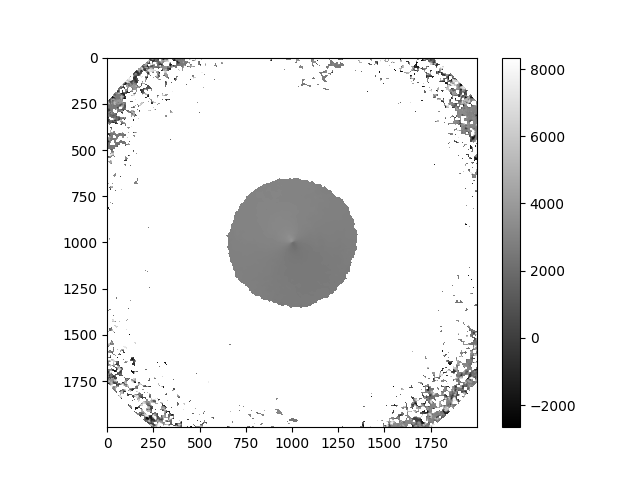
\includegraphics[width=\textwidth,height=\textheight,keepaspectratio]{fits_image_TWHya}
\label{fig:fig 1}
\end{figure}

\begin{figure}
\caption{FITS Image of HD16329}
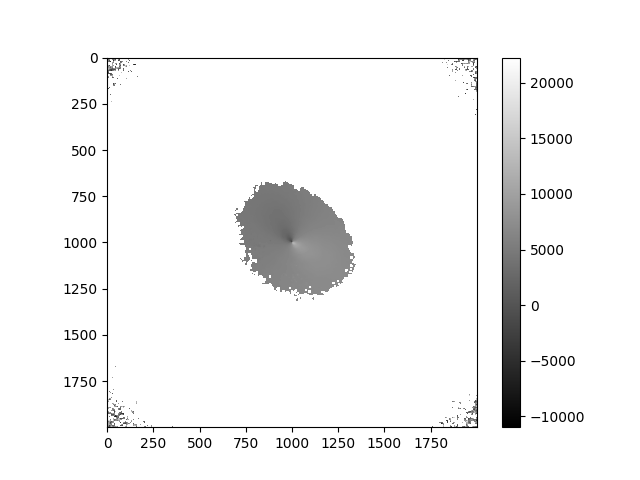
\includegraphics[width=\textwidth,height=\textheight,keepaspectratio]{fits_image_HD163296}
\label{fig:fig 2}
\end{figure}

\begin{figure}
\caption{Rotation Map of TW Hya}
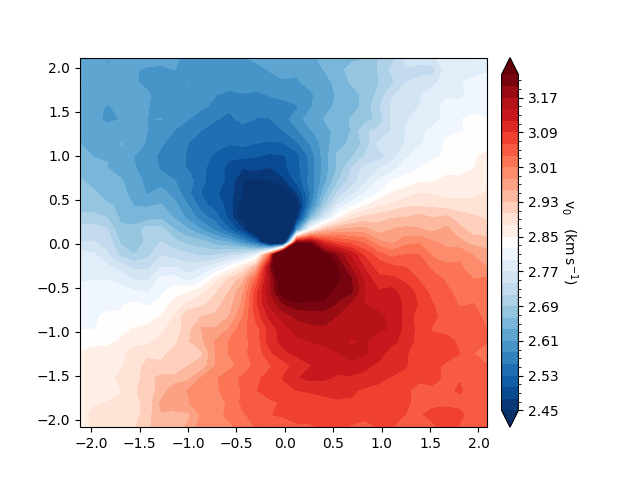
\includegraphics[width=\textwidth,height=\textheight,keepaspectratio]{TWHya_Rotate.png}
\label{fig:fig 3}
\end{figure}

\begin{figure}
\caption{Rotation Map of HD16329}
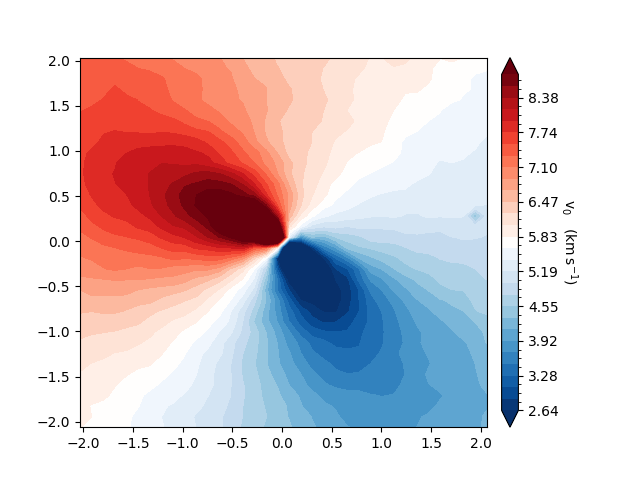
\includegraphics[width=\textwidth,height=\textheight,keepaspectratio]{HD163296_Rotate.png}
\label{fig:fig 4}
\end{figure}

\subsection{Task 2: Fitting the Rotation Map}
In this second task, the objective is to infer the geometrical properties by fitting a simple Keplerian rotation pattern to the measured rotation pattern. For the fitting, some of the parameters are fixed and guessed to obtain the source center, position angle, stellar mass, and the system velocity while holding the inclination fixed. The data is loaded from the intermediate file and runs through the package to return the statistics as a dictionary which is later saved in a CSV file for better readability. 

\begin{table}[ht]
\centering
\begin{tabular}{ |c|c| }
 \hline
 Source Center (x0, y0) & (-0.0031824375286493415, 0.01893629612535956) \\ 
 \hline
 Position angle of the disk (PA) & 151.1656724 \\ 
 \hline
  Stellar Mass (MSTAR) & 0.595716934 \\ 
 \hline
   Systemic Velocity (VLSR) & 2840.538396 \\ 
 \hline
\end{tabular}
\caption{Geometrical Properties of CO J = 2-1 observations of TW Hya}
\label{tab:table 1}
\end{table}

\begin{table}[ht]
\centering
\begin{tabular}{ |c|c| }
 \hline
 Source Center (x0, y0) & (-0.4224729691793593, 0.21709191610636597) \\ 
 \hline
 Position angle of the disk (PA) & 318.0026203 \\ 
 \hline
  Stellar Mass (MSTAR) & 2.924142732 \\ 
 \hline
   Systemic Velocity (VLSR) & 5935.563645 \\ 
 \hline
\end{tabular}
\caption{Geometrical Properties of CO J = 2-1 observations of HD16329}
\label{tab:table 2}
\end{table}

\section{Conclusion}
Therefore, the computational tasks were performed and the visualizations were saved into corresponding files. With the help of the software package, it was possible to plot a rotation map and fit it to obtain geometrical properties. The Astropy package helped read the FITS file and plot the data to get a snapshot of the initial map. 
\bibliographystyle{plain}
\bibliography{references}
\end{document}

